% !TeX encoding = UTF-8
% !TeX program = lualatex
% !TeX root = ../demo.tex
\begin{itemize}
\item
Air
\begin{itemize}
\item
\only<-?(Chameleo.0)>{\transparent{0.3}}
Chameleo
\item
\only<-?(Gannet.0)>{\transparent{0.3}}
Gannet
\end{itemize}
\item
\only<-?(Water.0)>{\transparent{0.3}}
Water
\begin{itemize}
\item
\only<-?(Octopus.0)>{\transparent{0.3}}
Octopus
\item
\only<-?(Starfish.0)>{\transparent{0.3}}
Starfish
\item
\only<?(PicassoTrans.range)>{\transparent{0.3}}
Picasso fish
\end{itemize}
\end{itemize}
%\endinput
\vbox to 0pt{\hbox{%
\only<?(Air.range)> {%
\tikz [
  remember picture,
  overlay,
] {
  \node [xshift=-\baselineskip] at (current page.east) [anchor = east,text width=0.4\textwidth] {
    \hfill\llap{%
      \visible<?(Chameleo.1)->{%
        \only<?(Gannet.1)->{\transparent{0.3}}
        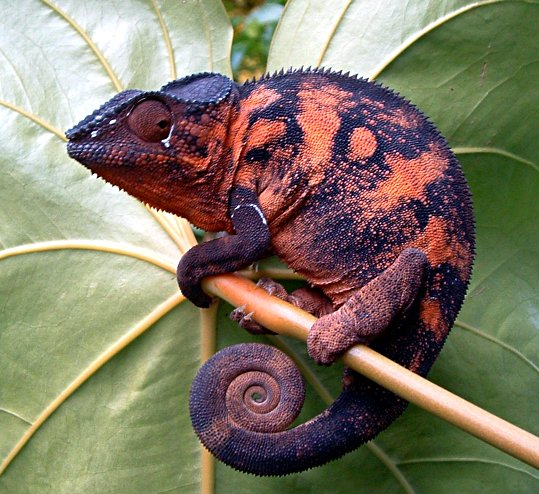
\includegraphics[width=\textwidth]{img/Air/Chameleon02}%
      }%
    }%
    \\[\baselineskip]
    \hfill\llap{%
      \visible<?(Gannet.1)->{%
        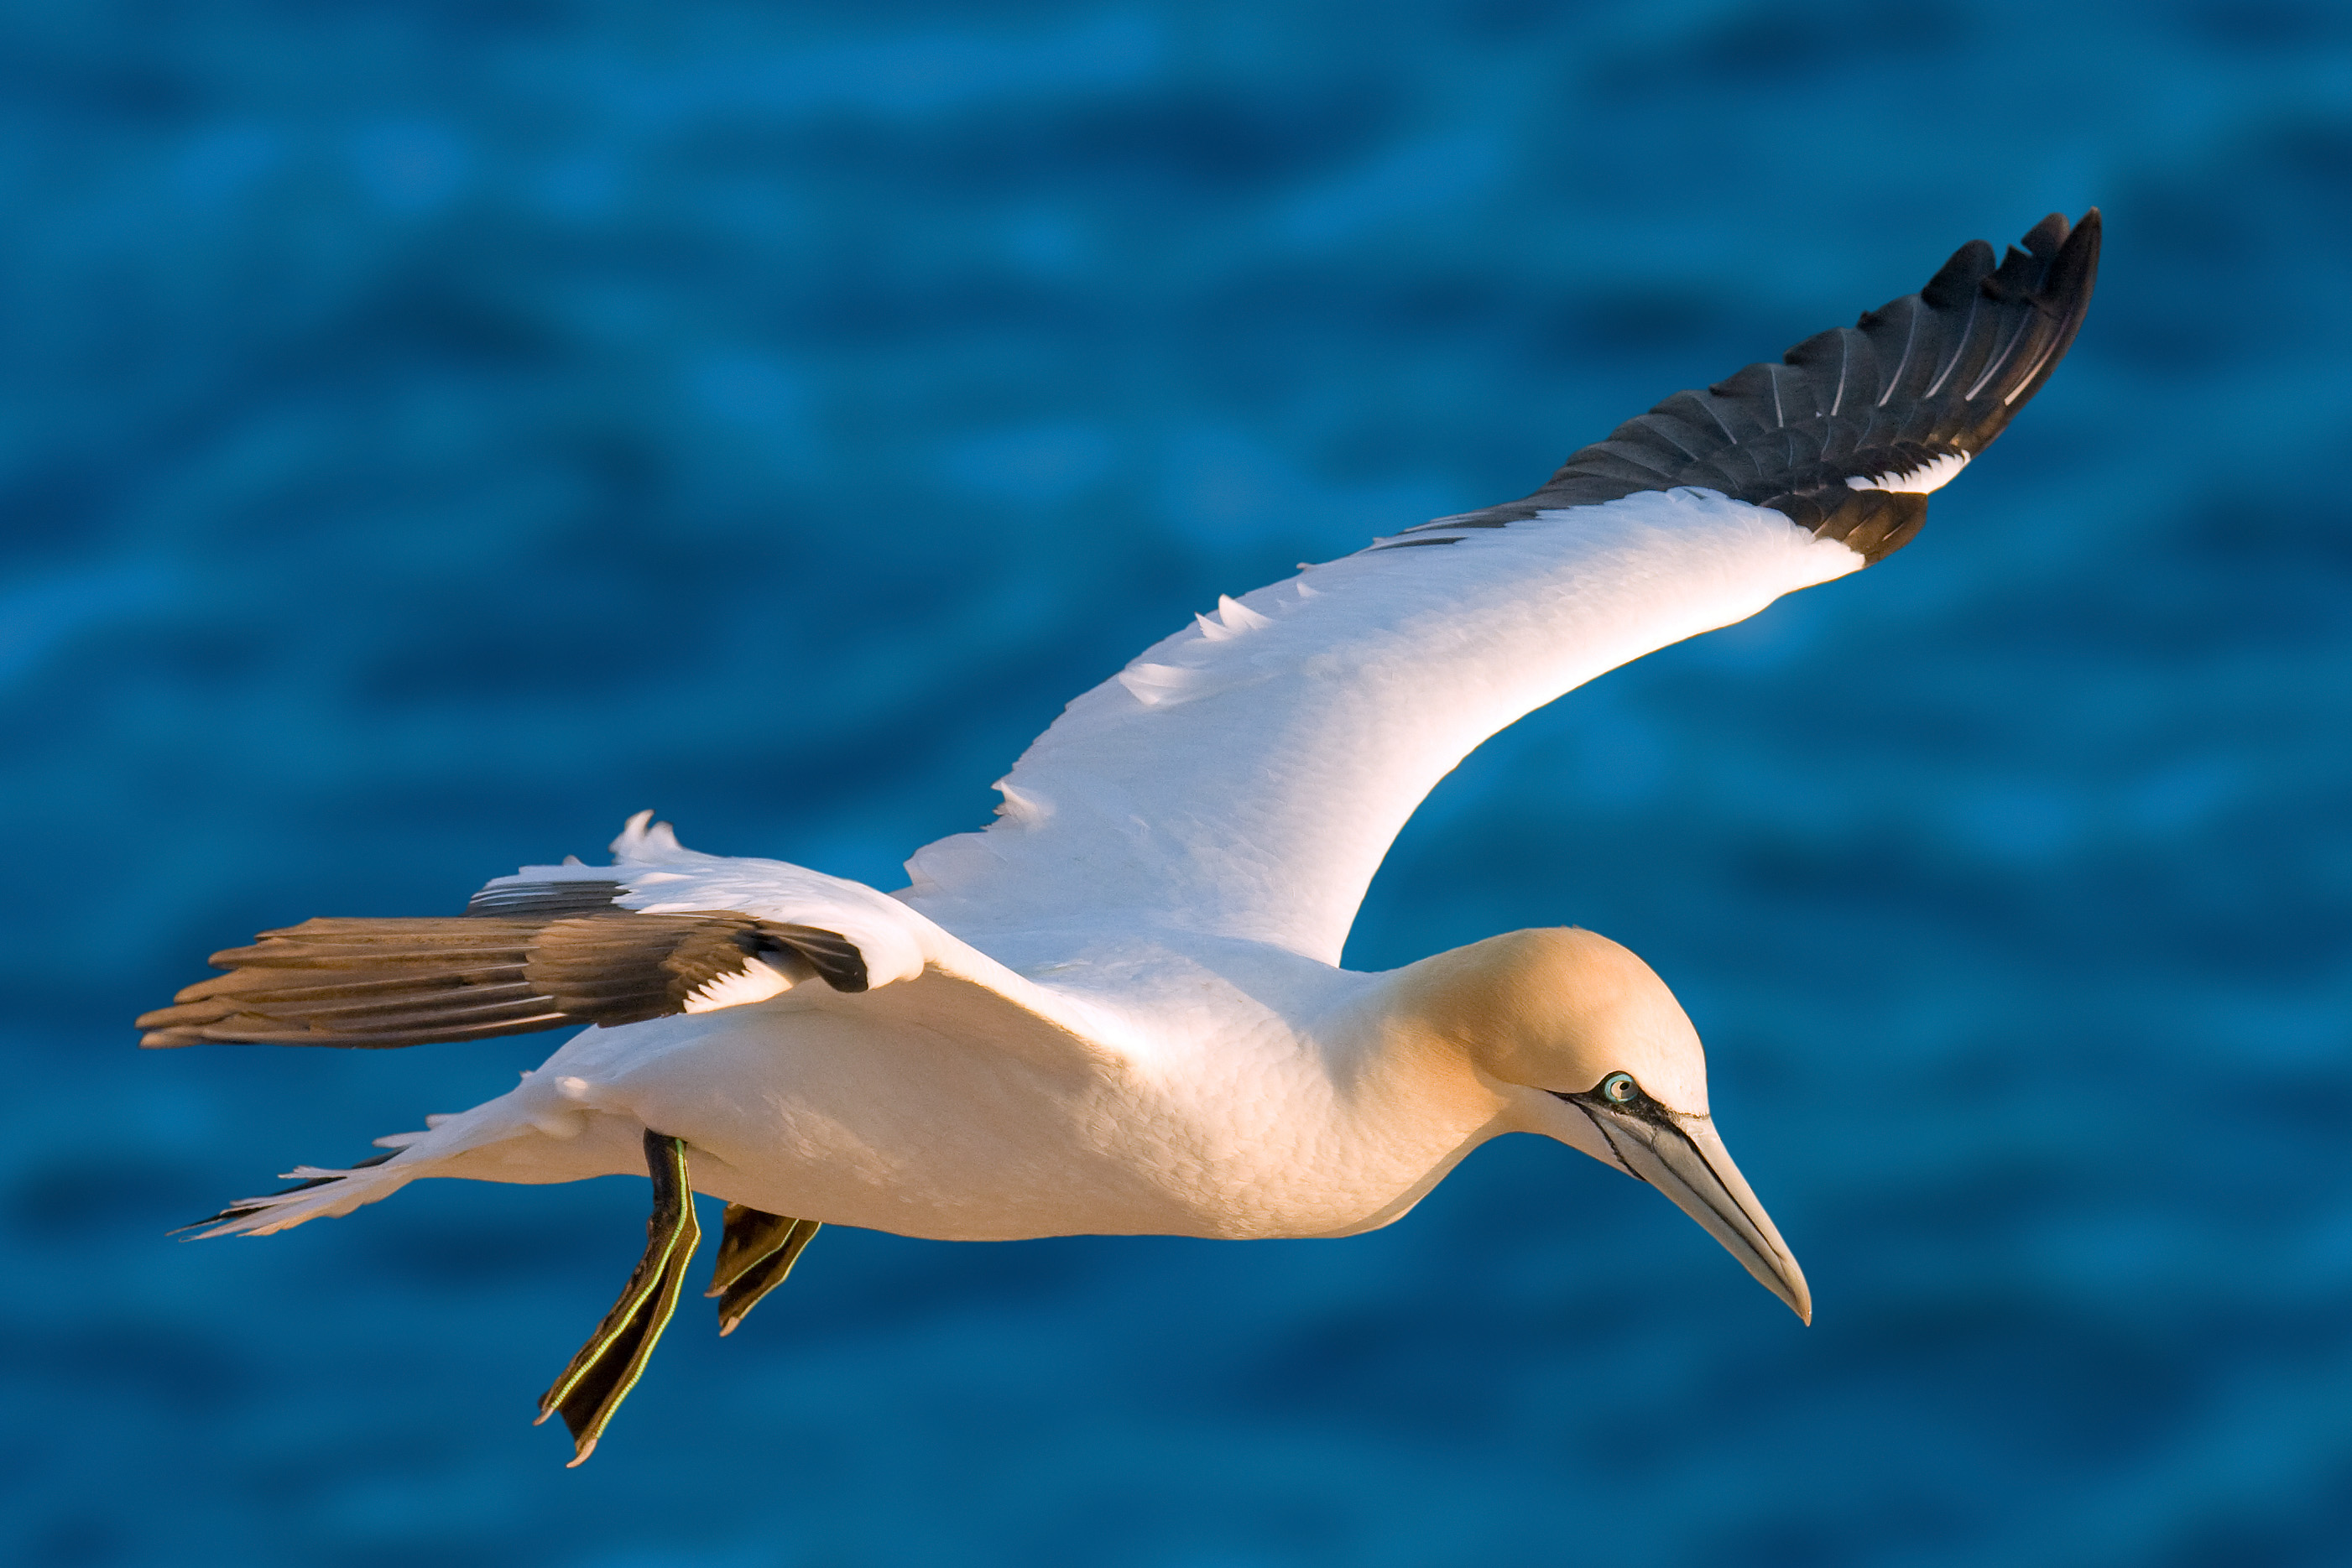
\includegraphics[width=\textwidth]{img/Air/Morus_bassanus_adu}%
      }%
    }%
  };
}%
}
\only<?(Water.range)> {%
\tikz [
  remember picture,
  overlay,
] {
  \node [xshift=-\baselineskip] at (current page.east) [anchor = east,text width=0.35\textwidth] {
    \hfill\llap{%
      \visible<?(Octopus.1)->{%
        \only<?(Starfish.1)->{\transparent{0.3}}
        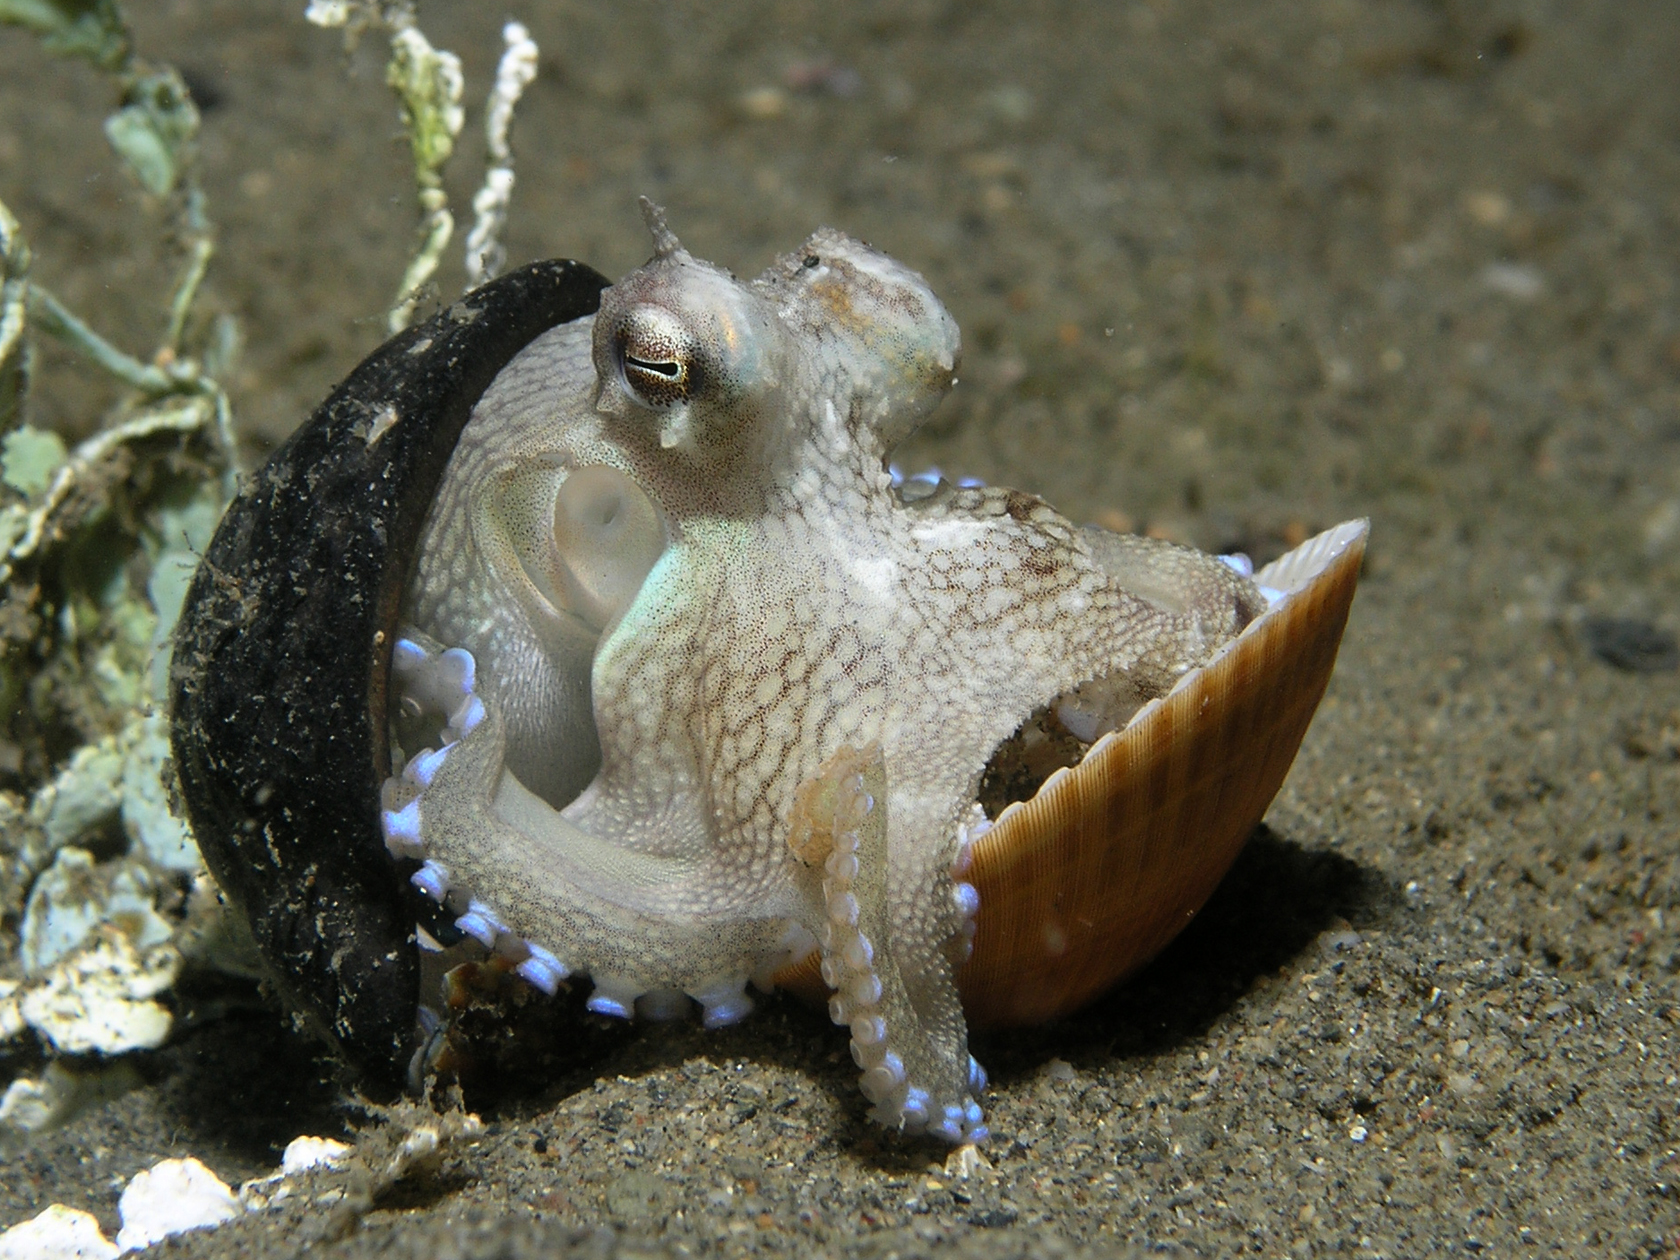
\includegraphics[width=\textwidth]{img/Water/Octopus_marginatus}%
      }%
    }%
    \\
    \vspace{-\baselineskip}%
    \hfill\llap{%
      \visible<?(Starfish.1)->{%
        \only<?(Picasso.range)>{\transparent{0.3}}
        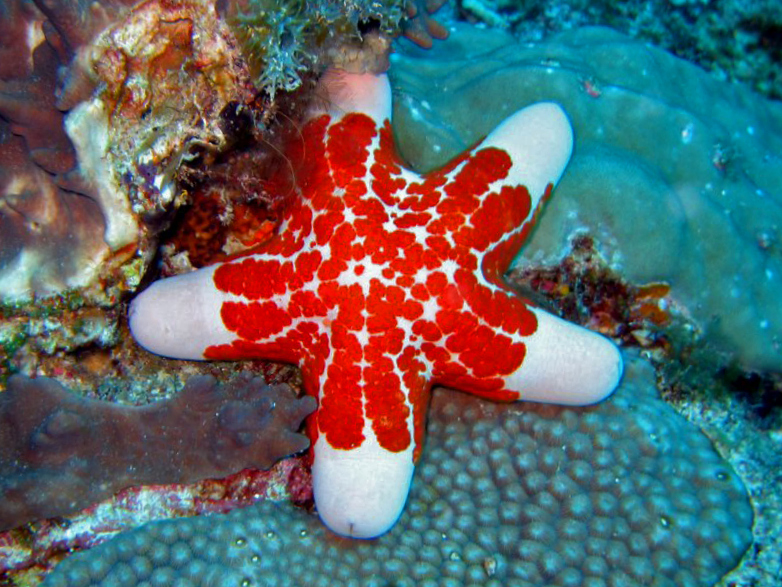
\includegraphics[width=\textwidth]{img/Water/Oreasteridae_-_Choriaster_granulatus}%
        \hspace{2\baselineskip}%
      }%
    }%
    \\
    \vspace{-\baselineskip}%
    \hfill\llap{%
      \visible<?(Picasso.range)>{%
        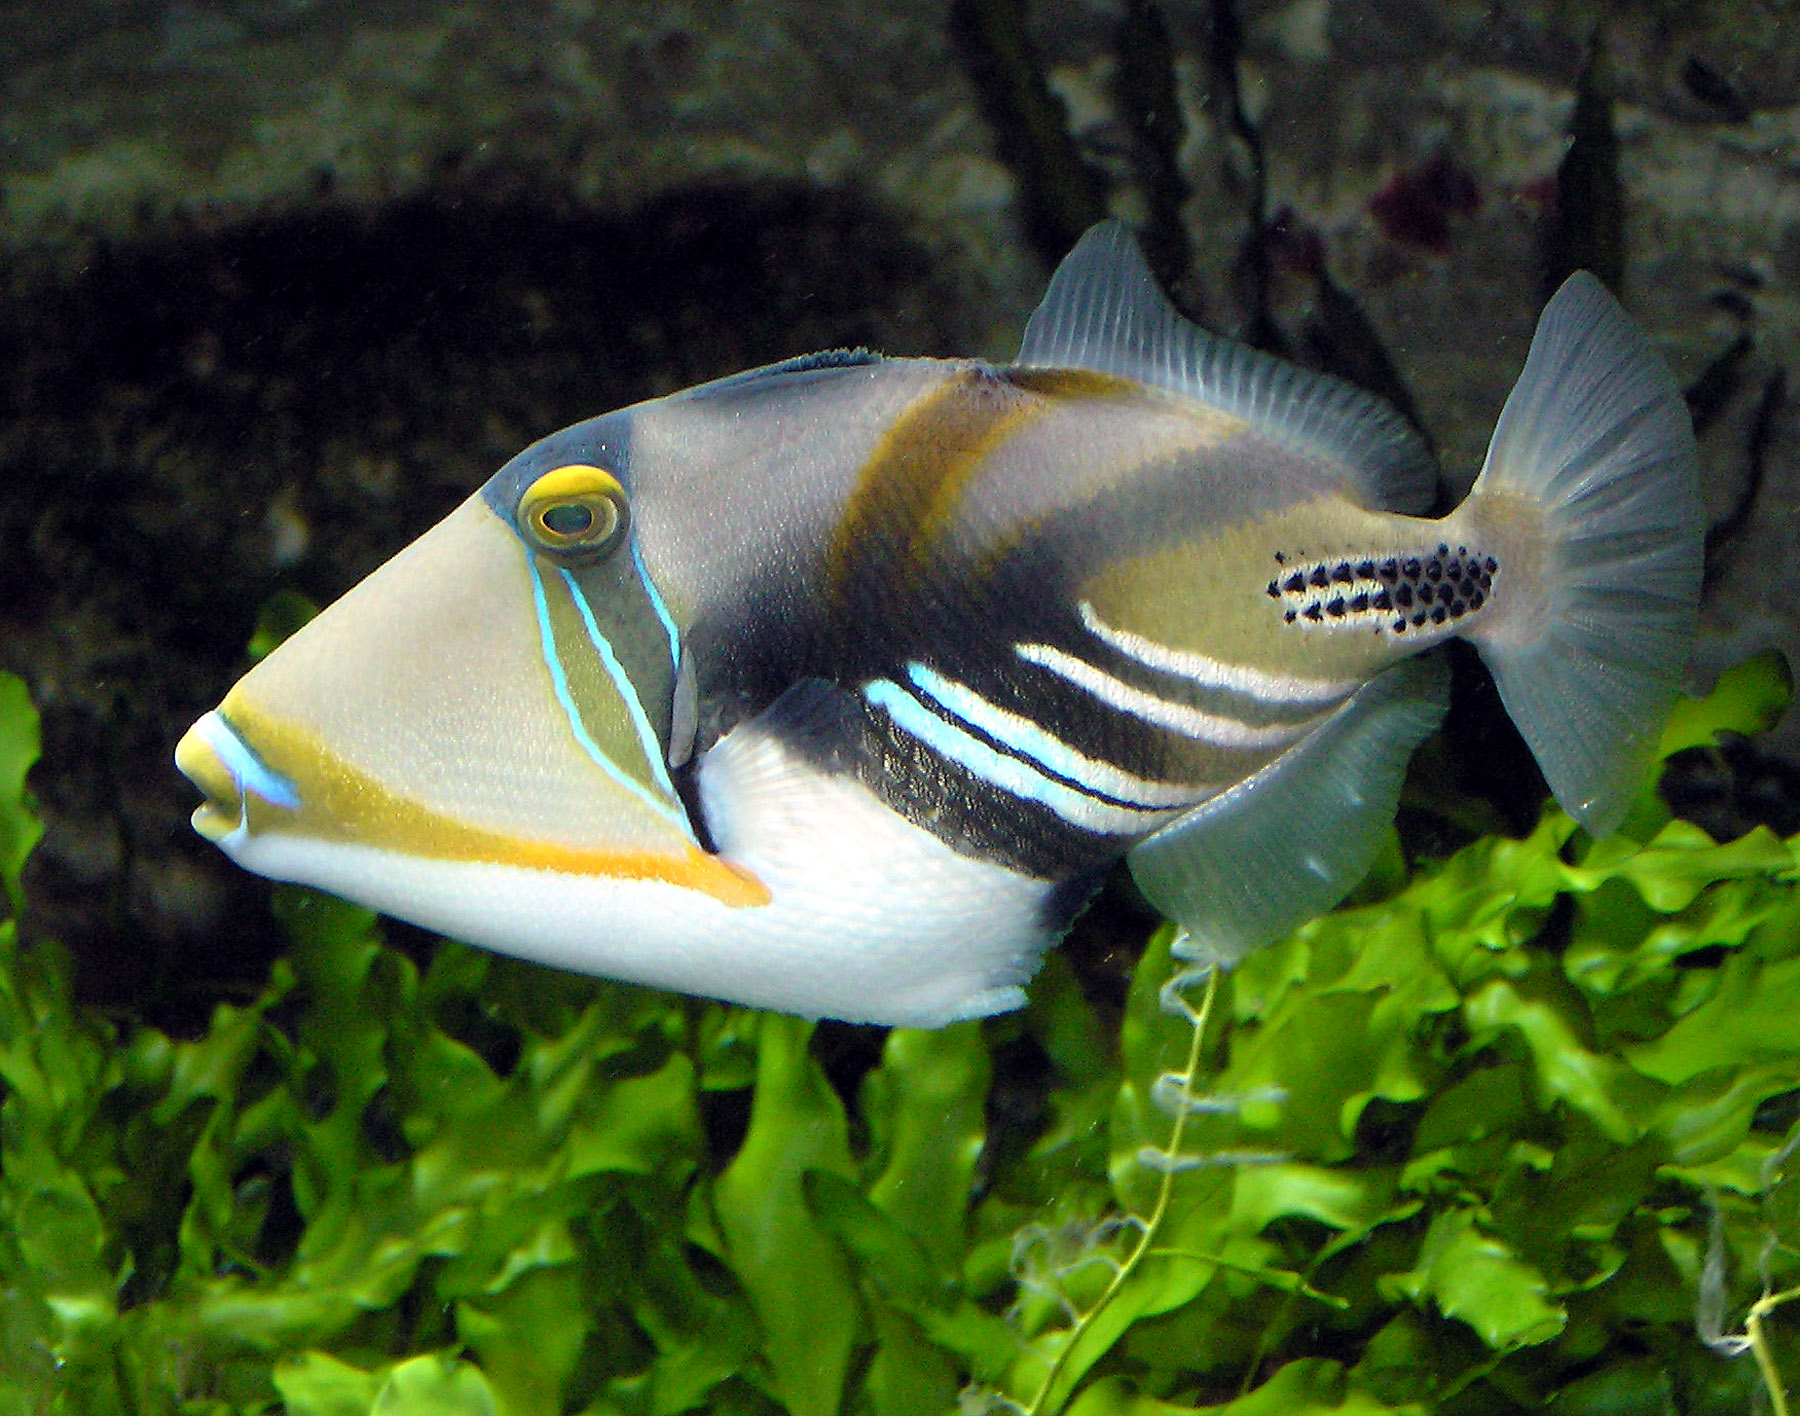
\includegraphics[width=\textwidth]{img/Water/Picasso.triggerfish.arp}%
      }%
    }%
  };
}%
}
\only<?(Summary.range)> {%
\tikz [
  remember picture,
  overlay,
] {
  \node [xshift=-\baselineskip] at (current page.east) [anchor = east,text width=0.275\textwidth] {%
    \hfill\llap{%
      \visible<?(Chameleo.1)->{%
        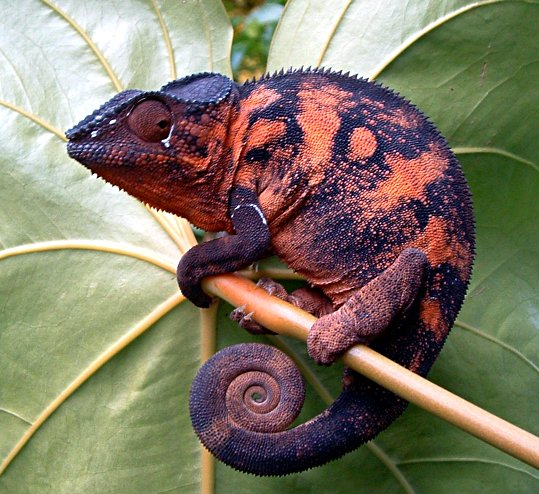
\includegraphics[width=\textwidth]{img/Air/Chameleon02}%
      }%
    }%
    \\\vspace{-0.5\baselineskip}%
    \hfill\llap{%
      \tblap{%
        \visible<?(Gannet.1)->{%
          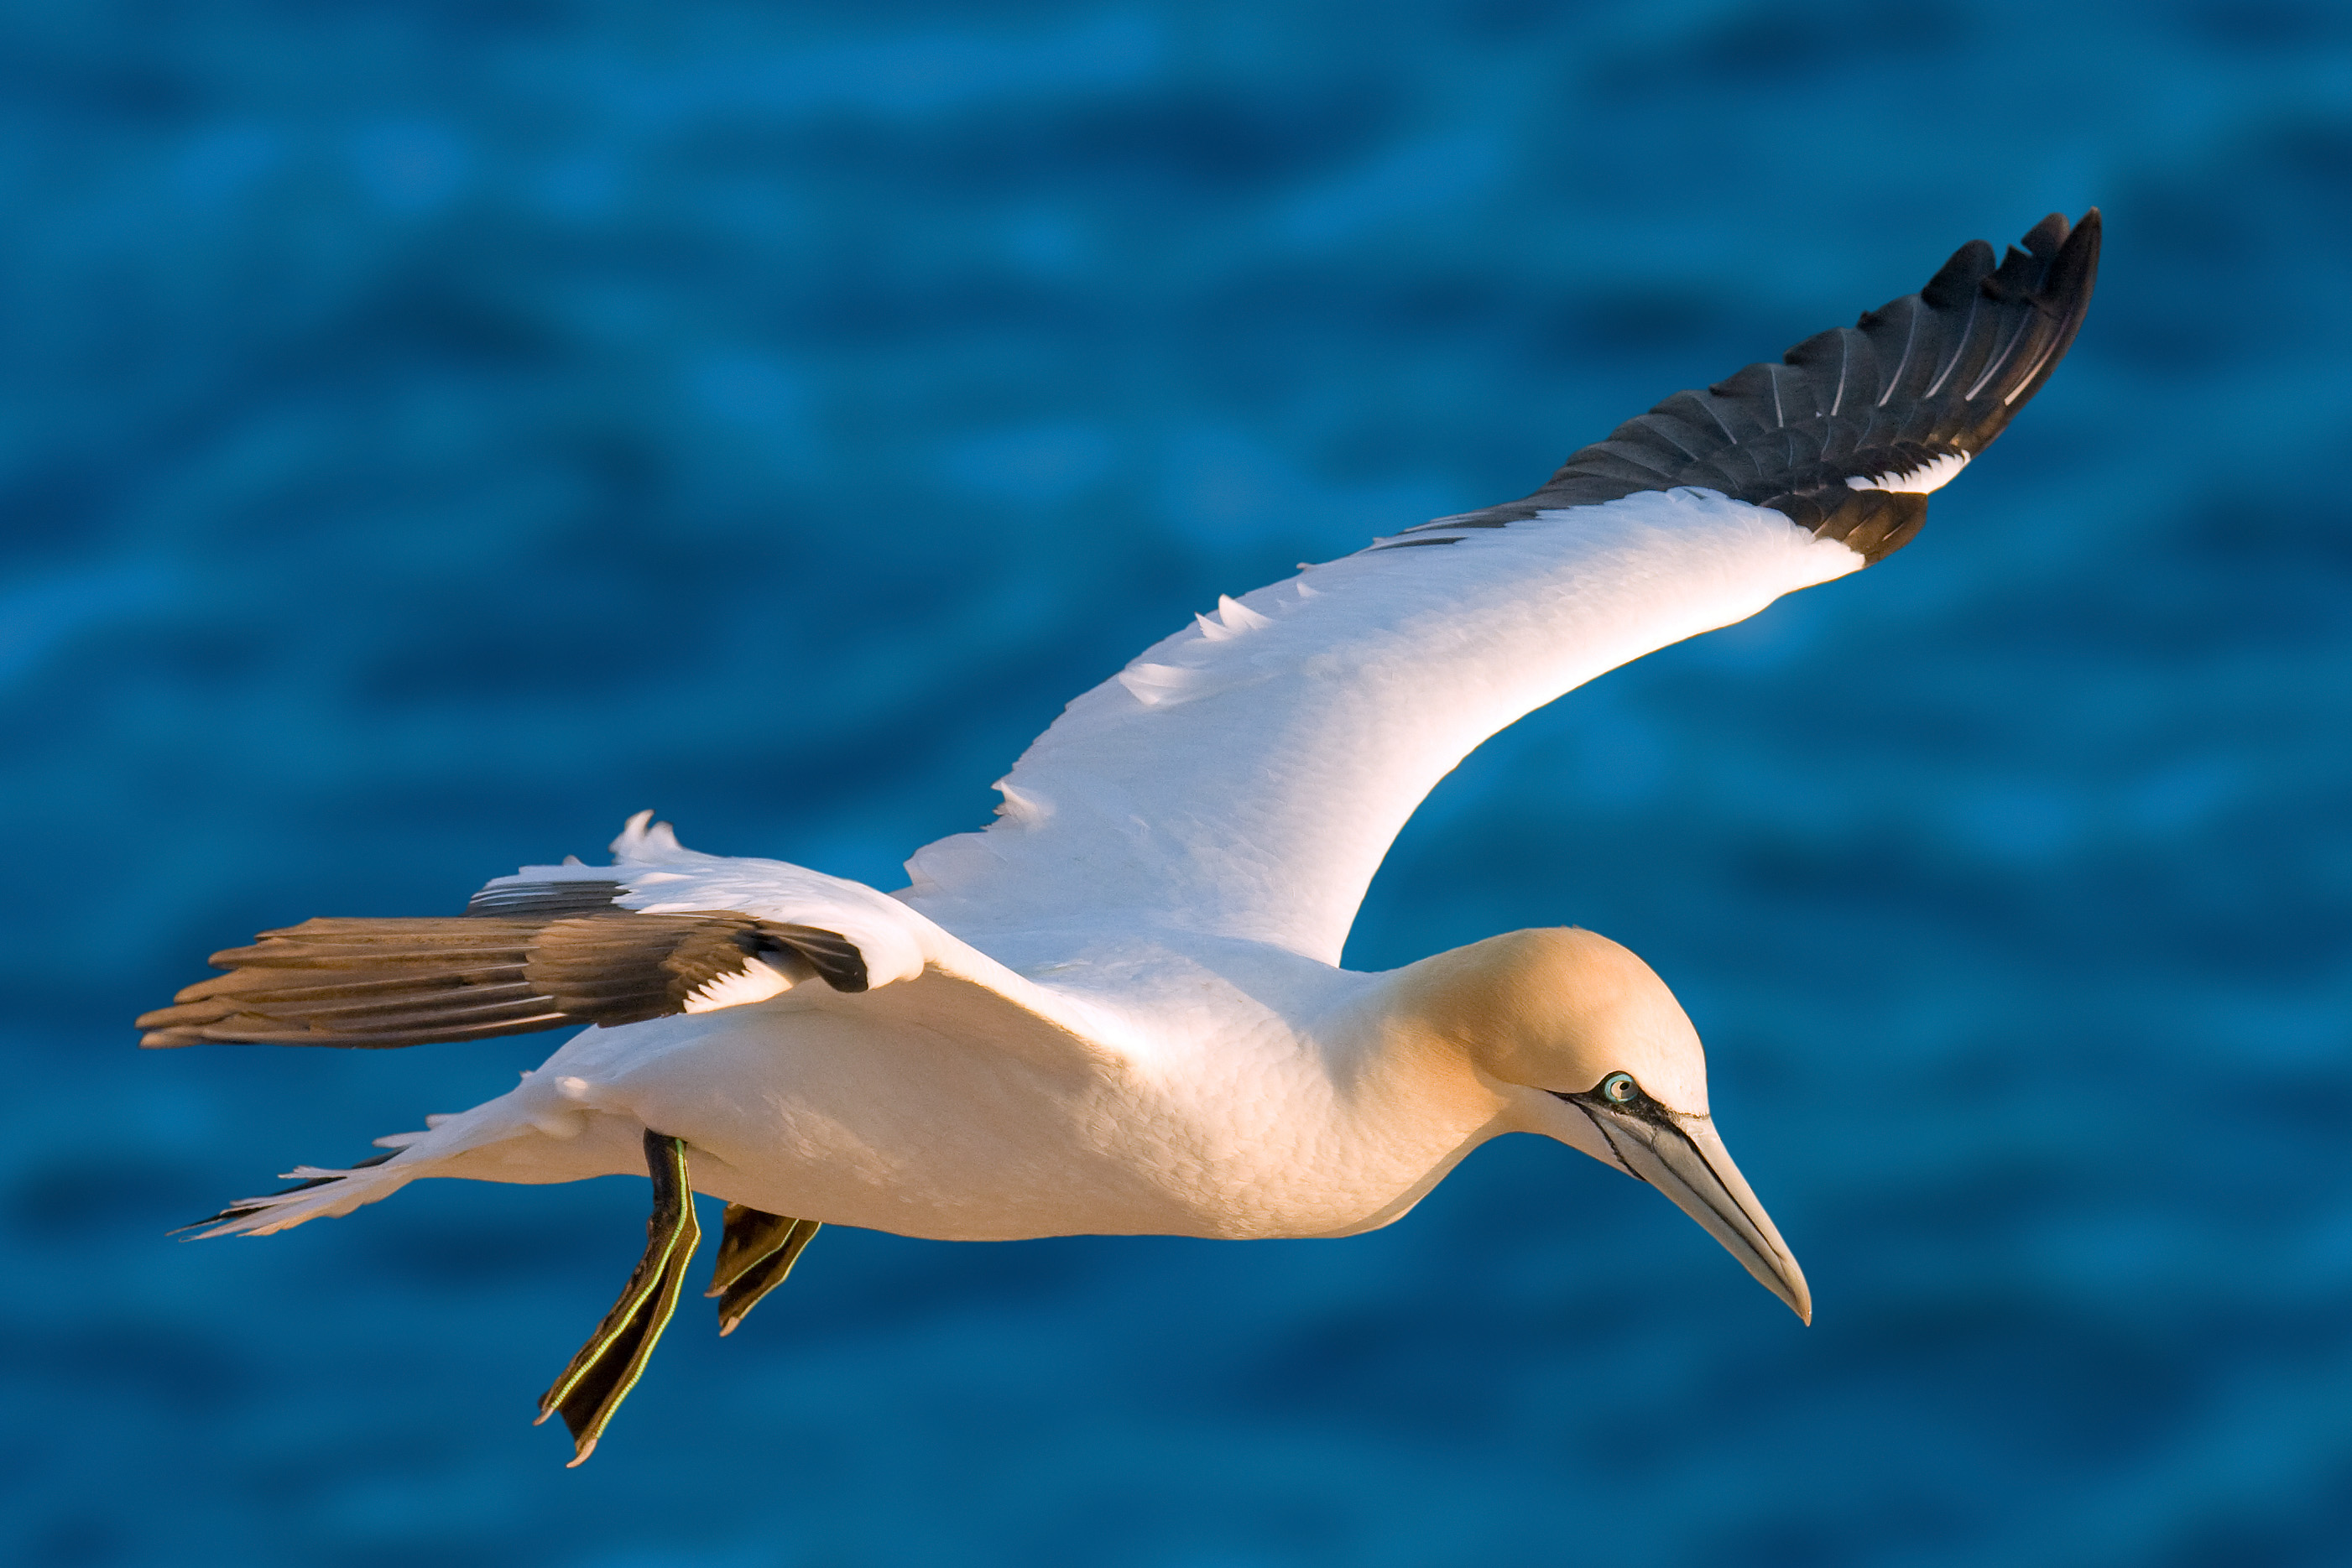
\includegraphics[width=\textwidth]{img/Air/Morus_bassanus_adu}%
          \hspace{6\baselineskip}%
        }%
      }%
    }%
    \\\vspace{-0.25\baselineskip}%
    \hfill\llap{%
      \visible<?(Octopus.1)->{%
        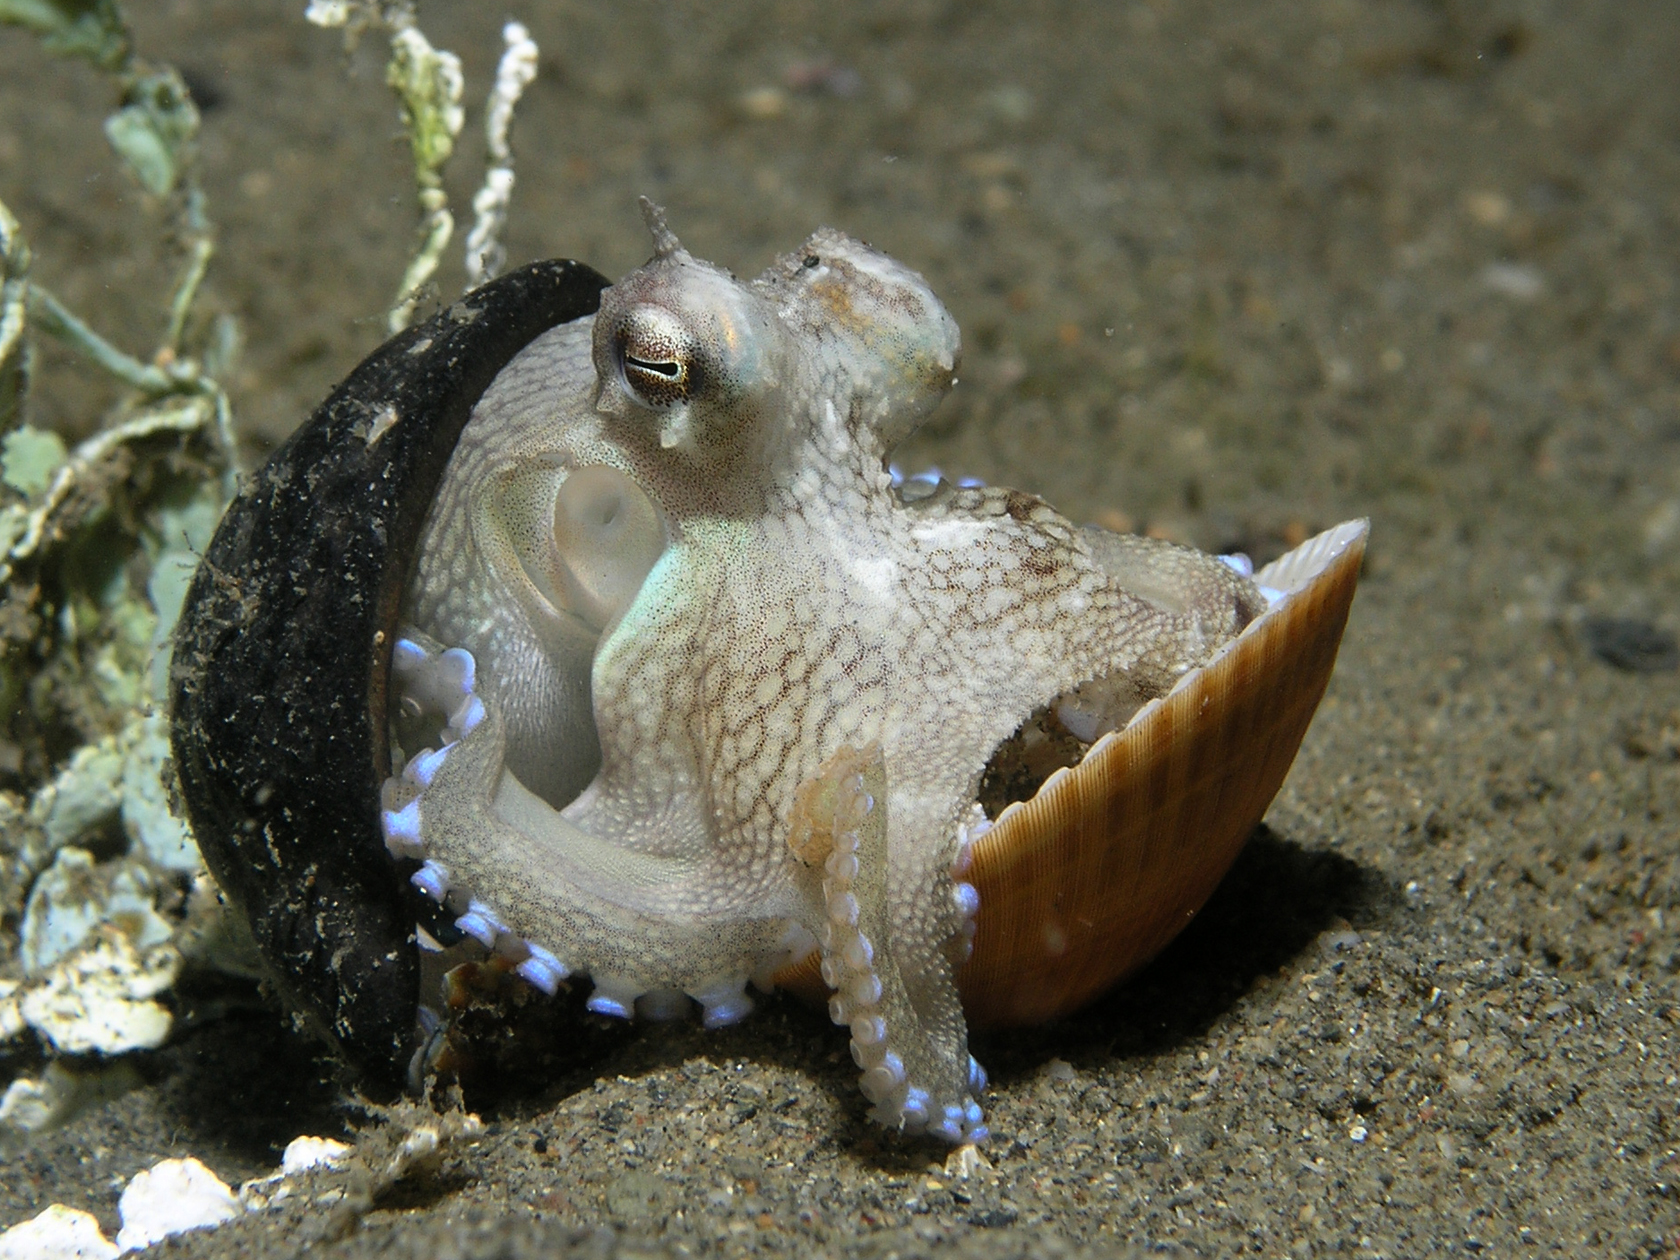
\includegraphics[width=\textwidth]{img/Water/Octopus_marginatus}%
        \hspace{0\baselineskip}%
      }%
    }%
    \\\vspace{-0.5\baselineskip}%
    \hfill\llap{%
      \tblap{%
        \visible<?(Starfish.1)->{%
          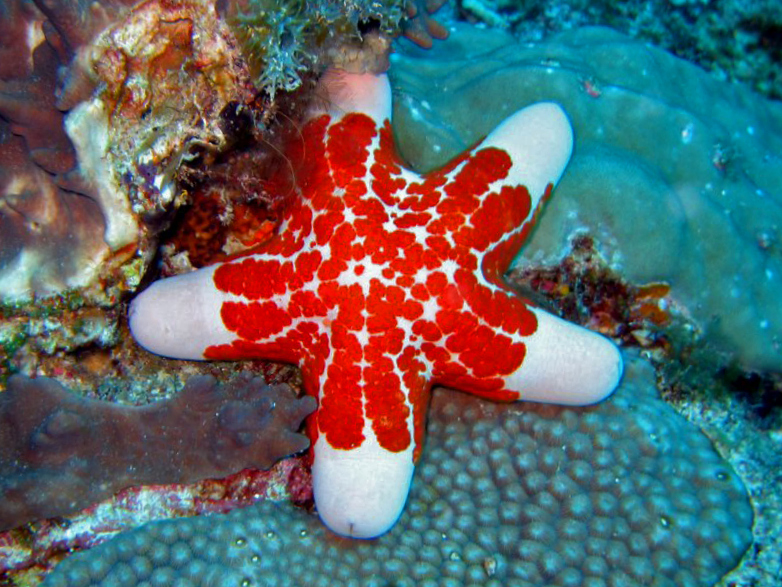
\includegraphics[width=\textwidth]{img/Water/Oreasteridae_-_Choriaster_granulatus}% 
          \hspace{6\baselineskip}%
        }%
      }%
    }%
    \\\vspace{-0.25\baselineskip}%
    \hfill\llap{%
      \visible<?(Picasso.1)->{%
        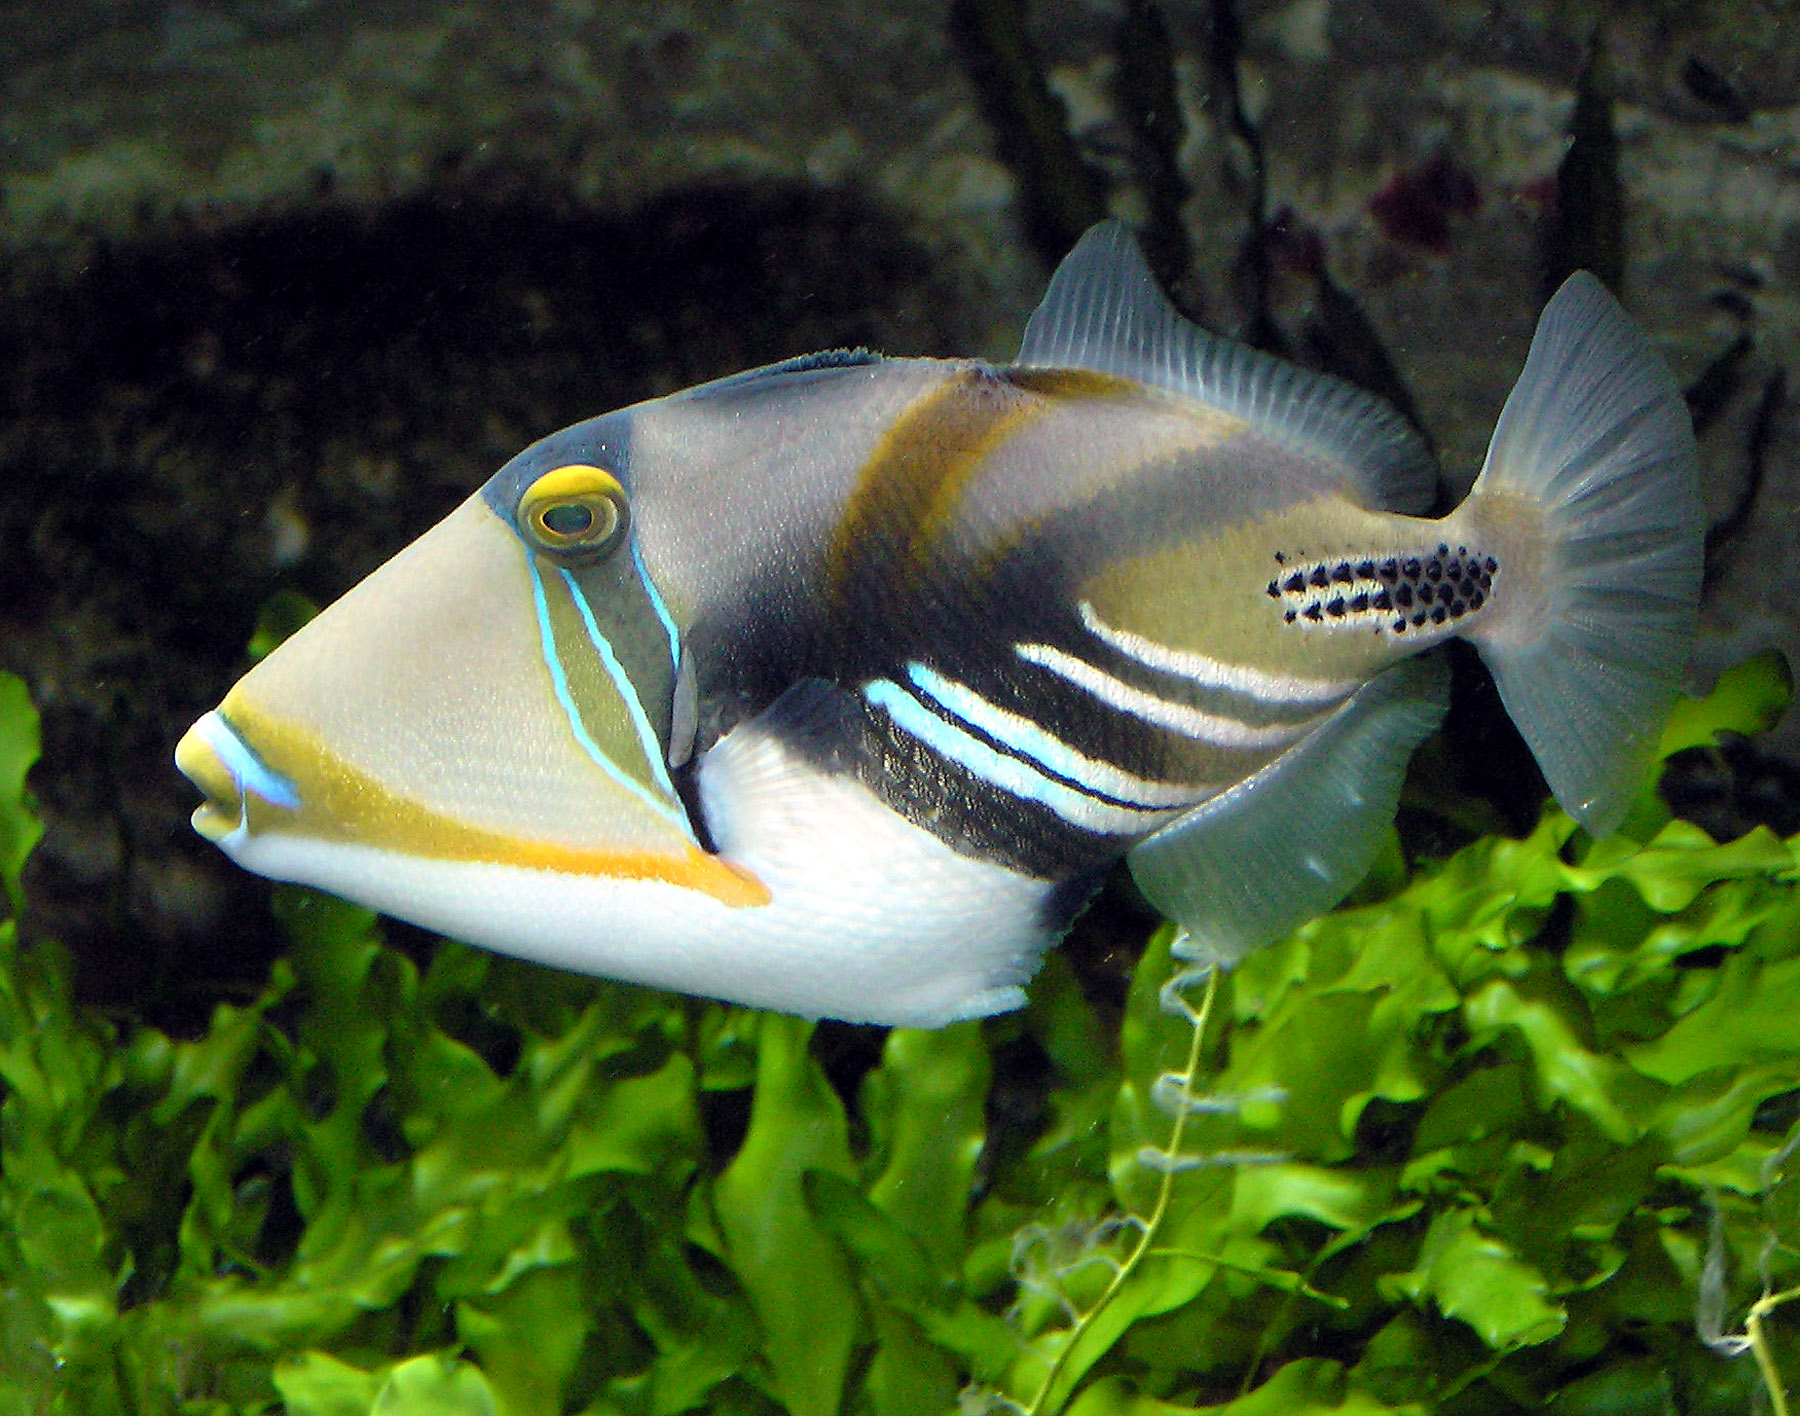
\includegraphics[width=\textwidth]{img/Water/Picasso.triggerfish.arp}%
      }%
    }%
  };
}%
}%
}}%
\Sticky<?(Air.last)>[anchor=south,yshift=1\baselineskip](current page.south){\bfseries
  Notice how the chameleon image is transparent%
}
\Sticky<?(StickyStarfish.range)>[anchor=south,yshift=1.5\baselineskip](current page.south){\bfseries Overlap allows for larger images}
